% Camera-Ready version of the paper.
%%%% Proceedings format for most of ACM conferences (with the exceptions listed below) and all ICPS volumes.
\documentclass[sigconf]{acmart}
%%%% As of March 2017, [siggraph] is no longer used. Please use sigconf (above) for SIGGRAPH conferences.

%%%% Proceedings format for SIGPLAN conferences
% \documentclass[sigplan, anonymous, review]{acmart}

%%%% Proceedings format for SIGCHI conferences
% \documentclass[sigchi, review]{acmart}

%%%% To use the SIGCHI extended abstract template, please visit
% https://www.overleaf.com/read/zzzfqvkmrfzn


\usepackage{booktabs} % For formal tables


% Copyright
\setcopyright{none}
%\setcopyright{acmcopyright}
%\setcopyright{acmlicensed}
% \setcopyright{rightsretained}
%\setcopyright{usgov}
%\setcopyright{usgovmixed}
%\setcopyright{cagov}
%\setcopyright{cagovmixed}


% DOI
% \acmDOI{10.475/123_4}

% ISBN
% \acmISBN{123-4567-24-567/08/06}

%Conference
\acmConference[PaPoC'18]{5th Workshop on Principles and Practice of Consistency for Distributed Data}{April 2018}{Porto, Portugal}
\acmYear{2018}
\copyrightyear{2018}

% \acmArticle{4}
% \acmPrice{15.00}

% These commands are optional
%\acmBooktitle{Transactions of the ACM Woodstock conference}
% \editor{Jennifer B. Sartor}
% \editor{Theo D'Hondt}
% \editor{Wolfgang De Meuter}


\begin{document}
\title{Improved Anti-Entropy with Reinforcement Learning}
% \titlenote{Produces the permission block, and copyright information}
% \subtitle{Extended Abstract}
% \subtitlenote{The full version of the author's guide is available as
%   \texttt{acmart.pdf} document}


\author{Benjamin Bengfort}
% \authornote{}
% \orcid{}
\affiliation{%
  \institution{University of Maryland}
% \streetaddress{}
% \city{College Park}
% \state{MD}
% \postcode{20742}
}
\email{bengfort@cs.umd.edu}

\author{Pete Keleher}
% \authornote{}
% \orcid{}
\affiliation{%
  \institution{University of Maryland}
% \streetaddress{}
% \city{College Park}
% \state{MD}
% \postcode{20742}
}
\email{keleher@cs.umd.edu}


\begin{abstract}
    Eventually consistent systems can be made more consistent by reducing the time
until a write is fully replicated, improving global visibility of updates.
While gossip-based anti-entropy methods scale well, random selection of
anti-entropy partners is less than efficient.
Moreover, while eventual consistency may be consistent enough in a single data
center, geographic replication increases visibility latency and leads to
externally observable inconsistencies.
In this paper, we explore an improvement to pairwise, bilateral anti-entropy;
instead of uniform random selection, we introduce reinforcement learning
mechanisms to assign selection probabilities to replicas most likely to have
information.
The result is more efficient replication, faster visibility, and stronger
eventual consistency while maintaining high availability and partition
tolerance.

\end{abstract}

%
% The code below should be generated by the tool at
% http://dl.acm.org/ccs.cfm
% Please copy and paste the code instead of the example below.
%
\begin{CCSXML}
<ccs2012>
<concept>
<concept_id>10010147.10010257.10010258.10010261</concept_id>
<concept_desc>Computing methodologies~Reinforcement learning</concept_desc>
<concept_significance>500</concept_significance>
</concept>
<concept>
<concept_id>10010520.10010575.10011743</concept_id>
<concept_desc>Computer systems organization~Fault-tolerant network topologies</concept_desc>
<concept_significance>500</concept_significance>
</concept>
<concept>
<concept_id>10010520.10010575.10010577</concept_id>
<concept_desc>Computer systems organization~Reliability</concept_desc>
<concept_significance>300</concept_significance>
</concept>
<concept>
<concept_id>10010520.10010575.10010578</concept_id>
<concept_desc>Computer systems organization~Availability</concept_desc>
<concept_significance>300</concept_significance>
</concept>
</ccs2012>
\end{CCSXML}

\ccsdesc[500]{Computing methodologies~Reinforcement learning}
\ccsdesc[500]{Computer systems organization~Fault-tolerant network topologies}
\ccsdesc[300]{Computer systems organization~Reliability}
\ccsdesc[300]{Computer systems organization~Availability}


\keywords{Eventual Consistency, Anti-Entropy, Reinforcement Learning}


\maketitle

\section*{Introduction}

A distributed system is made highly available when individual servers are
allowed to operate independently without failure-prone, high latency
coordination.
The independent nature of the server's behavior means that it can immediately
respond to client requests, but that it does so from a limited, local
perspective which may be inconsistent with another server's response.
If individual servers in a system were allowed to remain wholly independent,
individual requests from clients to different servers would create a lack of
order or predictability, a gradual decline into inconsistency, e.g. the
system would experience \textit{entropy}.
To combat the effect of entropy while still remaining highly available,
servers engage in periodic background \textit{anti-entropy
  sessions}~\cite{terry_session_1994}.

Anti-entropy sessions synchronize the state between servers ensuring that,
at least briefly, the local state is consistent with a portion of the global
state of the system.
If all servers engage in anti-entropy sessions, the system is able to make
some reasonable guarantees about consistent replication; the most famous
of which is that without requests the system will become
globally consistent, eventually~\cite{vogels_eventually_2009}.
More specifically, inconsistencies in the form of stale reads can be bound by
likelihoods that are informed by the latency of anti-entropy sessions and the
size of the system~\cite{bailis_probabilistically_2012,bailis_quantifying_2014}.
Said another way, overall consistency is improved in an eventually consistent
system by decreasing the likelihood of a stale read, which is tuned by
improving the \textit{visibility latency} of a write, the speed at which a
write is propagated to a significant portion of servers.
This idea has led many system designers to decide that eventual consistency
is ``consistent enough''~\cite{bermbach_eventual_2011,wada_data_2011},
particularly in a data center context where visibility latency is far below
the rate of client requests, leading to practically strong consistency.

However, there has been an important change in considerations for the
design of such systems that have led us to re-evaluate propagation speed:
systems are growing, while simultaneously becoming geographically distributed
outside of datacenters.
Large geographically-distributed systems are becoming the norm particularly
as mobile devices and sensor systems participate in computing and storage at
the edge of large distributed
systems~\cite{garcia_lopez_edge-centric_2015,scellato_track_2011}.
From content delivery systems that span the globe, to mobile applications, to
future systems such as automated vehicular networks, all will require
additional consistency guarantees without sacrificing availability.
However, scaling an eventually consistent system to dozens or even hundreds
of nodes increases the radius of the network, which leads to increased noise
during anti-entropy e.g. the possibility that an anti-entropy session will be
between two already synchronized nodes.
Geographic distribution and extra-datacenter networks also increase the
latency of anti-entropy sessions so that inconsistencies become more apparent
to external observers.

We address the challenge of large, geographically distributed eventually
consistent systems by improving synchronization using reinforcement
learning techniques.
Anti-entropy uses gossip and rumor spreading to propagate updates
deterministically without saturating the
network even in the face of network
outages~\cite{haeupler_simple_2015,karp_randomized_2000,moreno_dynamics_2004}.
These protocols use uniform random selection to choose synchronization peers,
which means that a write occurring at one replica is not efficiently
propagated across the network.
In this paper we explore the use of \textit{multi-armed bandit}
algorithms~\cite{langford_epoch-greedy_2008,luo_efficient_2017} to optimize
for fast, successful synchronizations by modifying peer selection
probabilities.
The result is a synchronization topology that emerges according to access
patterns and network latency which produces efficient synchronization,
localizes most data exchange, lowers visibility latency and increases
consistency.

Our contribution for this early stage work is a demonstration of the
potential for replicas to meaningfully influence global consistency by
modifying local behavior in response to their computing environment.
This potential has been motivated by our larger work which investigates the
effect of scaling systems, both in terms of size and distance, on consistency.
We show this potential though experiments run on a system with dozens of
replica distributed across 5 continents which show that even a relatively
simple implementation of adaptivity leads to a pronounced benefit in
visibility latency, and therefore the overall consistency of the system.


\section*{Background}

Our investigation considers an eventually consistent, in-memory key-value
store that is totally replicated using
anti-entropy~\cite{decandia_dynamo:_2007}.
A brief description of the system and consistency considerations follows.

\subsection*{Accesses and Consistency}

Clients can \texttt{Put} (write) and \texttt{Get} (read) key-value pairs to
 and from one or more replicas in a single operation.
The set of replicas that responds to a client creates a quorum that must
agree on the state of the operation at its conclusion.
Clients can vary read and write quorum sizes to improve consistency or
availability -- larger quorums reduce the likelihood of inconsistencies
caused by concurrent updates, but smaller quorums respond much more quickly,
particularly if the replicas in the quorum are co-located with the client.
In large, geo-replicated systems we assume that clients will prefer to choose
fewer, local replicas to connect with, optimistic that collisions across the
wide-area are rare, e.g. that writes are localized but reads are global.

On \texttt{Put}, the instance of the key-value pair created by the update is
assigned a monotonically increasing, conflict-free \textit{version
number}~\cite{parker_detection_1983,almeida_version_2002}.
For simplicity, we assume a fixed number of replicas, therefore each version
is made up of two components: the \textit{update} and \textit{precedence ids}.
Precedence ids are assigned to replicas during configuration, and update ids
are incremented to the largest observed value during synchronization.
As a result, any two versions generated by a \texttt{Put} anywhere in the
system are comparable such that the \textit{latest} version of the key-value
pair is the version with the largest update id, and in the case of ties, the
largest precedence id.

Additional version metadata, including the parent version of the update (in a
read-then-write system or simply the latest version of the key stored
locally), implements a virtual object history that allows us to reason about
consistency.
Keys can be managed independently, e.g. each key has its own update id
sequence resulting in per-object consistency, or all objects can be managed
together with a single sequence; in the latter case, it is possible to
construct an ordering history of operations to all objects and in the former,
a sequence of operations for each object.
Object histories allow us to reason about the global consistency of the
system.

There are two primary inconsistencies that can occur in this system:
\textit{stale reads} and \textit{forked writes}.
A stale read means that the \texttt{Get} operation has not returned
the globally most recent version of the object, e.g. the local replica is
behind in the object history.
A forked write is caused when there are two concurrent writes to the same
object, a symptom of stale reads.
Forked writes cause a divergence in the object history such that there are
two or more branches of update operations.
As we will see in the next section, one of these writes will eventually be
\textit{stomped} before it can become fully replicated, meaning that the
eventual consistency prunes these branches at the cost of losing
the update.
The ideal consistency for a system is represented by a linear object history
without forks~\cite{bernstein_rethinking_2013}, which demonstrates that the
system was in a consistent state during all accesses.

Both forms of inconsistency can be primarily attributed to \emph{visibility
latency}, that is the time it takes for an update to propagate to all
replicas in the system.
Visibility latency is directly related to the likelihood of stale reads with
respect to the frequency of accesses~\cite{bailis_quantifying_2014}; said
another way, decreasing the visibility latency improves the overall
consistency of a system.
However, in a system that uses anti-entropy for replication, the propagation
speed of an update is not governed solely by network connections, it is also
bound to the number and frequency of anti-entropy sessions conducted and the
radius of the network.

\subsection*{Anti-Entropy}

Anti-entropy sessions are conducted in a pairwise fashion on a periodic
interval to ensure that the network is not saturated with synchronization
requests which may reduce client availability.
At each interval, every replica selects a synchronization partner such that
all replicas have a uniform likelihood of selection.
This ensures that an update originating at one replica will be propagated to
all online replicas given the continued operation of replication.
This mechanism also provides robustness in the face of failure; a single
unresponsive replica or even network partition does not become a bottleneck
to synchronization, and once the failure is repaired synchronization will
occur without reconfiguration.

There are two basic forms of synchronization: \textit{push} synchronization
is a fire-and-forget form of synchronization where the remote is sent the
latest version of all objects, whereas \textit{pull} synchronization requests
the latest version of objects and minimizes the size of data transfer.
To get the benefit of both, we consider \textit{bilateral} synchronization
which combines push and pull in a two-phase exchange.
Bilateral synchronization increases the effect of anti-entropy during each
exchange because it ensures that in the common case each replica is
synchronized with two other replicas instead of one during every anti-entropy
period.

Bilateral anti-entropy starts with the initiating replica sending a vector of
the latest local versions of all keys currently stored, usually optimized
with Merkel or prefix trees to make comparisons faster.
The remote replica compares the versions sent by the initiating replica with
its current state and responds with any objects whose version is
\textit{later} than the initiating replica's as well as another version
vector of requested objects that are earlier on the remote.
The initiating replica then replies with the remote's requested objects,
completing the synchronization.
We refer to the first stage of requesting later objects from the remote as
the pull phase, and the second stage of responding to the remote the push
phase.

There are two important things to note about this form of anti-entropy
exchange.
First, this type of synchronization implements a \textit{latest writer wins}
policy.
This means that not all versions are guaranteed to become fully replicated
-- if a later version is written during propagation of an earlier version,
then the earlier version gets \emph{stomped} by the later version because
only the latest versions of objects are exchanged.
If there are two concurrent writes, only one write will become fully
replicated, the write on the replica with the greater precedence.
Second, visibility latency is maximized when all replicas choose a remote
synchronization partner that does not yet have the update.
This means that maximal visibility latency is equal to $t\log_3n$, where
$t$ is the anti-entropy interval and $n$ is the number of replicas in the
network.
In practice, however, because of inefficient exchanges due to uniform random
selection of synchronization partners, this latency is never practically
achieved, and is instead modulated by a noise variable that is
proportional to the size of the network.

\section*{Bandit Approaches}

To combat the effect of noise on visibility latency our initial approach
employs a technique commonly used in active and reinforcement learning:
multi-armed bandits.
Multi-armed bandits refer to a statistical optimization procedure that is
designed to find the optimal payout of several choices that each have
different probabilities of reward.
In this case, we use bandits to improve uniform random selection of peers so
that replicas choose synchronization partners that are most likely to exchange
information and thus more quickly propagate updates, while still maintaining
the properties of full replication and fault tolerance.

A bandit problem is designed by identifying several (usually more than two)
competing choices called ``arms''\footnote{Arms refer to the pulling
mechanism of a slot machine, the metaphor generally used to motivate the
multi-armed bandit problem.}, as well as a reward function that determines how
successful the selection of an arm is.
During operation, the bandit selects an arm, observes the rewards, then
updates the payout likelihood of the selected arm, normalized by the number
of selections.
As the bandit selects arms, it learns which arm or arms have the highest
likelihood of reward, and can modify it's arm selection \emph{strategy} to
maximize the total reward over time.

Bandits must balance exploration of new arms with possibly better reward
values and exploitation of an arm that has higher rewards than the other.
In the \emph{epsilon greedy strategy}, the bandit will select the arm with
the best reward with some probability $1-\epsilon$, otherwise it will select
any of the arms with uniform probability.
The smaller $\epsilon$ is, the more the bandit favors exploitation of known
good arms, the larger $\epsilon$ is, the more it favors exploration.
If $\epsilon=1$ then the algorithm is simply uniform random selection.
A simple extension of this is a strategy called \emph{annealing epsilon
greedy}, which starts with a large $\epsilon$, then as the number of trials
increases, steadily decreases $\epsilon$ on a logarithmic scale.
There are many other bandit strategies but we have chosen these two simple
strategies for our initial research to demonstrate a bolt-on effective
improvement to existing systems.

\begin{table}[h]
\centering
\begin{tabular}{@{}l c c c @{}}
\toprule
& \textbf{Pull} & \textbf{Push} & \textbf{Total} \\
\midrule
Synchronize at least 1 object & 0.25 & 0.25 & 0.50 \\
Synchronize multiple objects  & 0.05 & 0.05 & 0.10 \\
Latency $\leq$ 5ms (local)        & 0.10 & 0.10 & 0.20 \\
Latency $\leq$ 100ms (regional)   & 0.10 & 0.10 & 0.20 \\
\midrule
\textit{Total} & \textit{0.50} & \textit{0.50} & \textit{1.00} \\
\bottomrule
\end{tabular}
\caption{Reward Function}
\label{tab:rewards}
\end{table}

Peer selection for anti-entropy is usually conducted with uniform random
selection to guarantee complete replication.
To extend anti-entropy with bandits, we design a selection method whose arms
are remote peers and whose rewards are determined by the success of
synchronization.
The goal of adding bandits to anti-entropy is to optimize selection of peers
such that the visibility latency becomes closer to the optimal propagation
time as a synchronization topology emerges from the bandits.
A secondary goal is to minimize anti-entropy latency by preferring local (in
the same data center) and regional (e.g. on the same continent) connections.

Our initial reward function favors synchronizations to replicas where the
most writes are occurring by giving higher rewards to anti-entropy sessions
that exchange later versions in either a push or a pull as well as additional
rewards if more than one object is exchanged.
Additionally, the latency of the synchronization RPCs is computed to reward
replicas that are near each other.
The complete reward function is given in Table~\ref{tab:rewards}: for each
phase of synchronization (push and pull), compute the reward as the sum of the
propositions given.
For example if a synchronization results in three objects being pulled in
250ms, and one object being pushed in 250ms, the reward is 0.75.

The design of reward functions can be implemented to the needs of a specific
system.
For example, in a system that has workloads with variable sized writes, object
size could be considered or systems with imbalanced deployments might
consider a reward function that prioritizes inter-region communication.

\section*{Experiments}

\begin{figure}[b]
    \centering
    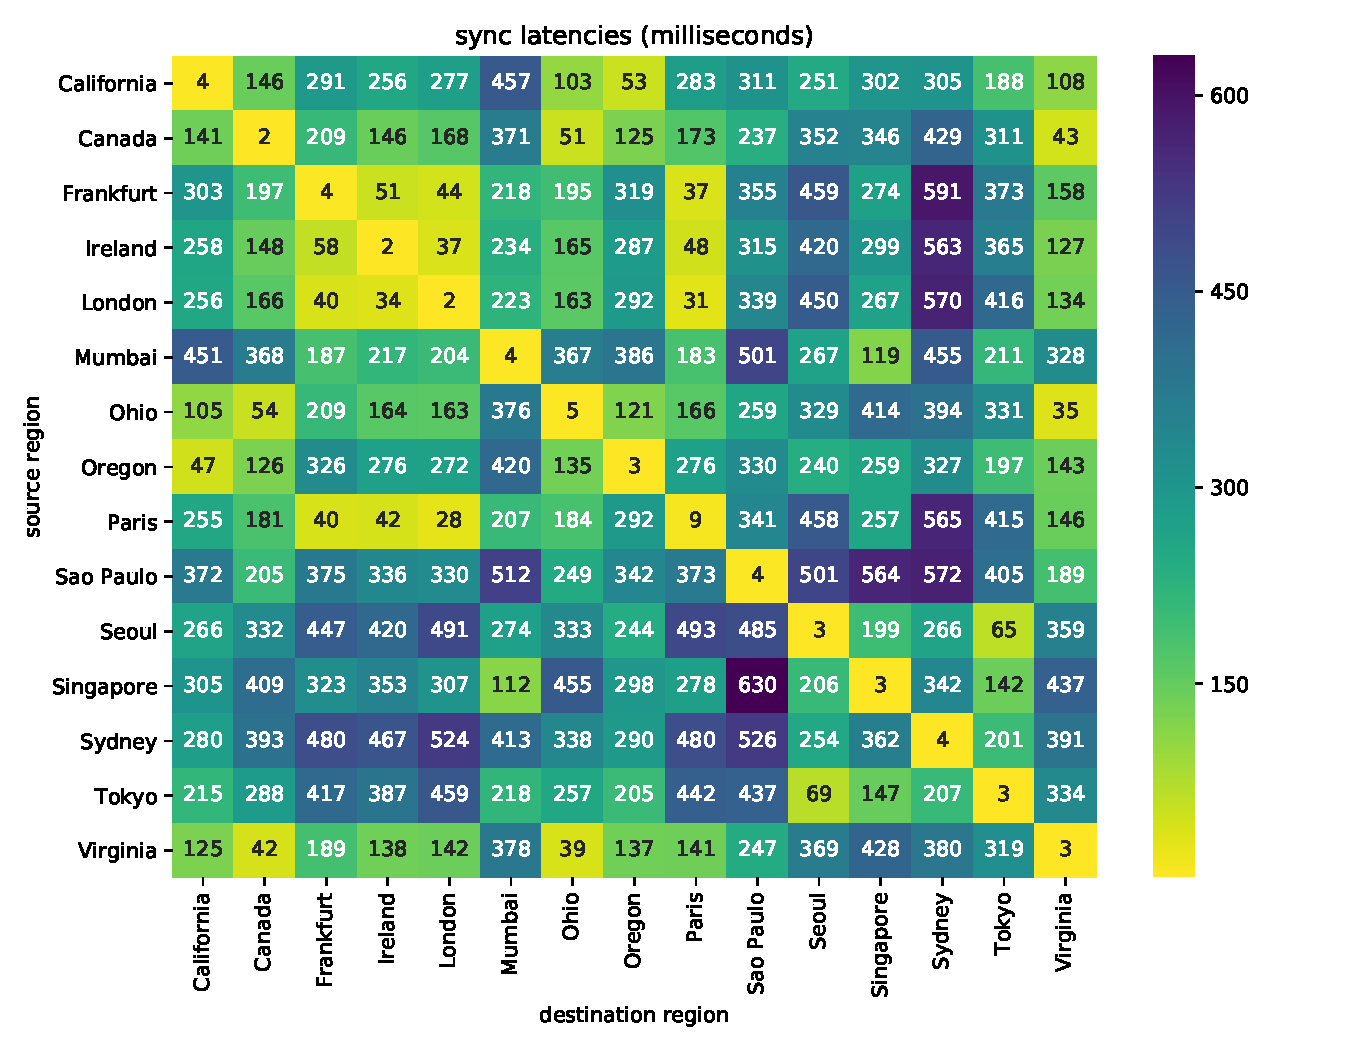
\includegraphics[width=0.5\textwidth]{figures/latency_sync_heatmap}
    \caption{Inter-Region Synchronization Latencies (Push+Pull)}
    \label{fig:latency_sync_heatmap}
\end{figure}

\begin{figure*}[t]
    \centering
    \minipage{0.5\textwidth}
      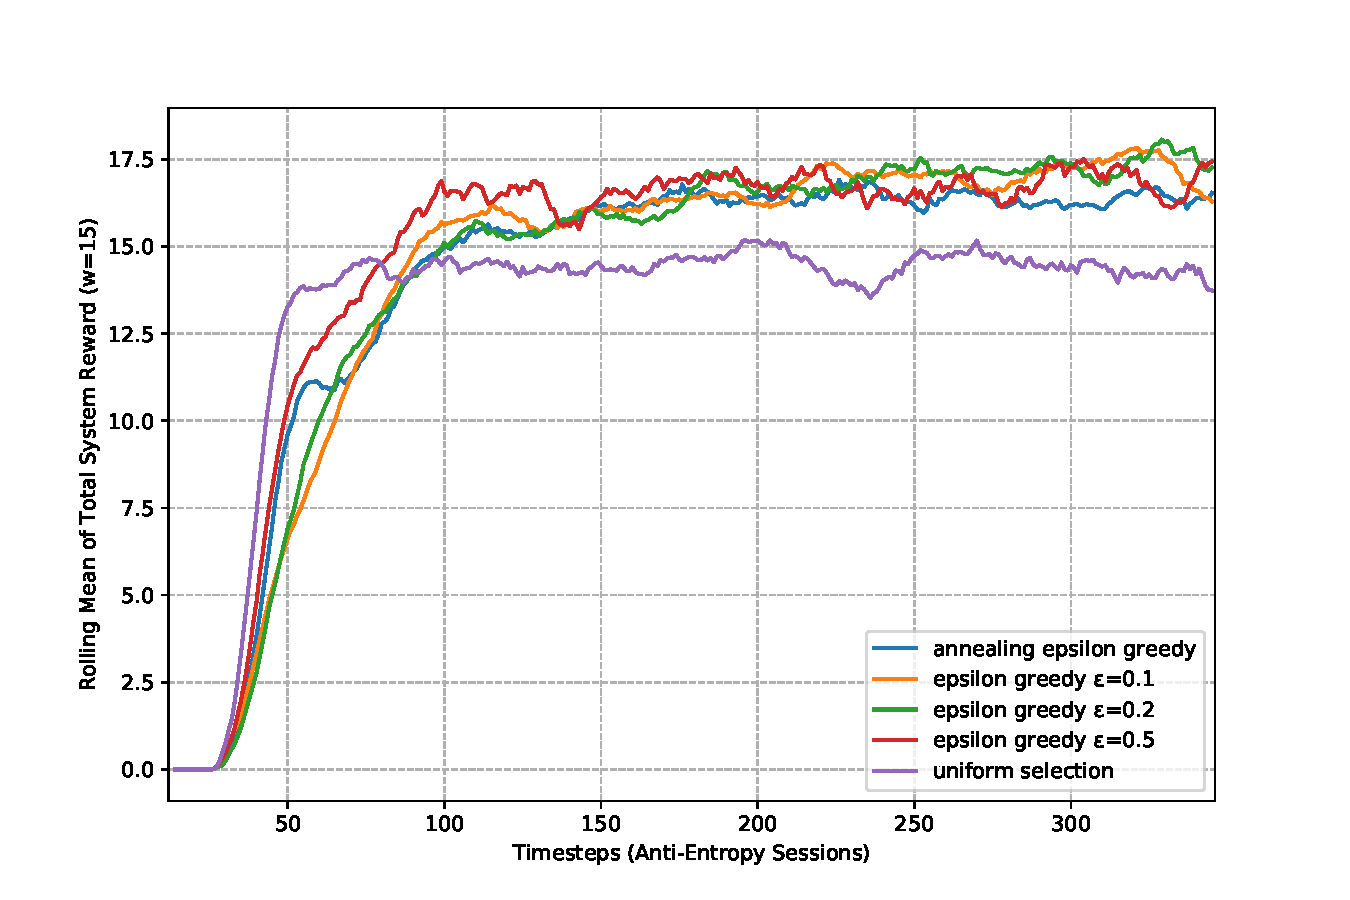
\includegraphics[width=\linewidth]{figures/rewards}
      \caption{Total system rewards over time}
      \label{fig:system_rewards}
    \endminipage\hfill
    \minipage{0.5\textwidth}%
      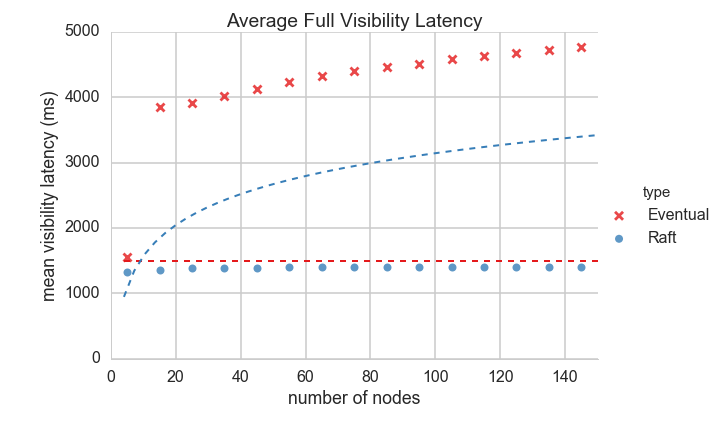
\includegraphics[width=\linewidth]{figures/visibility_latency}
      \caption{Visibility Latency by Region}
      \label{fig:visibility_latency}
    \endminipage
\end{figure*}

We conducted experiments using a distributed key-value store totally
replicated across 45 replicas in 15 geographic regions on 5 continents
around the world.
Replicas were hosted using AWS EC2 t2.micro instances and were connected to
each other via internal VPCs when in the same region, using external
connections between regions.
The store, called Honu, is implemented in Go 1.9 using gRPC and protocol
buffers for RPC requests; all code is open source and available on GitHub.

The workload on the system was generated by 15 clients, one in each region and
colocated with one of the replicas.
Clients continuously created Put requests for random keys with a unique
prefix per-region such that consistency conflicts only occur within a
single region.
The average throughput generated per-client was 5620.4 puts/second.
The mean synchronization latency between each region ranged from 35ms to
630ms, shown in~\ref{fig:latency_sync_heatmap}, because of this we set the
anti-entropy interval to 1 second to train the system, then set the interval
to 125ms to measure visibility latency.
To account for lag between commands sent to replicas in different regions,
each experiment was run for 11 minutes, the bandit learning period was 4
minutes then visibility latency was observed for 6 minutes, buffered by 30
seconds before and after the workload to allow replicas to initialize and
gracefully shutdown.

Our first experiments compared uniform random peer selection with epsilon
greedy bandits using $\epsilon \in \{0.1, 0.2, 0.5\}$ as well as an annealing
epsilon greedy bandit.
The total system rewards as a rolling mean over a time window of 20
synchronizations are shown in Figure~\ref{fig:system_rewards}.
The rewards ramp up from zero as the clients come online and start
creating work to be synchronized.
All of the bandit algorithms eventually improve over the baseline of uniform
selection, not only generating more total reward across the system, but also
introducing less variability in rewards over time.
None of the bandit curves immediately produces high rewards as they explore
the reward space; lower $\epsilon$ values may cause exploitation of incorrect
arms, while higher $\epsilon$ values take longer to find optimal topologies.
However, in the static workload case, the more aggressive bandit strategies
converge more quickly to the optimal reward.

Visibility latencies were computed by reducing the workload rate to once
every 4 seconds to ensure the write becomes fully visible across the entire
network.
During the visibility measurement period, replicas logged the timestamp the
write was pushed or pulled, and the visibility latency is computed as the
difference between the minimum and maximum timestamp.
Both the visibility latency and the average number of anti-entropy sessions
are shown in Figure~\ref{fig:visibility_latency}.
Employing bandit strategies reduces the visibility latency from 2360ms on
average in the uniform case to 1870ms, reducing the number of required
anti-entropy intervals by approximately 4.

\begin{figure*}[t]
    \centering
    \minipage{0.33\textwidth}
      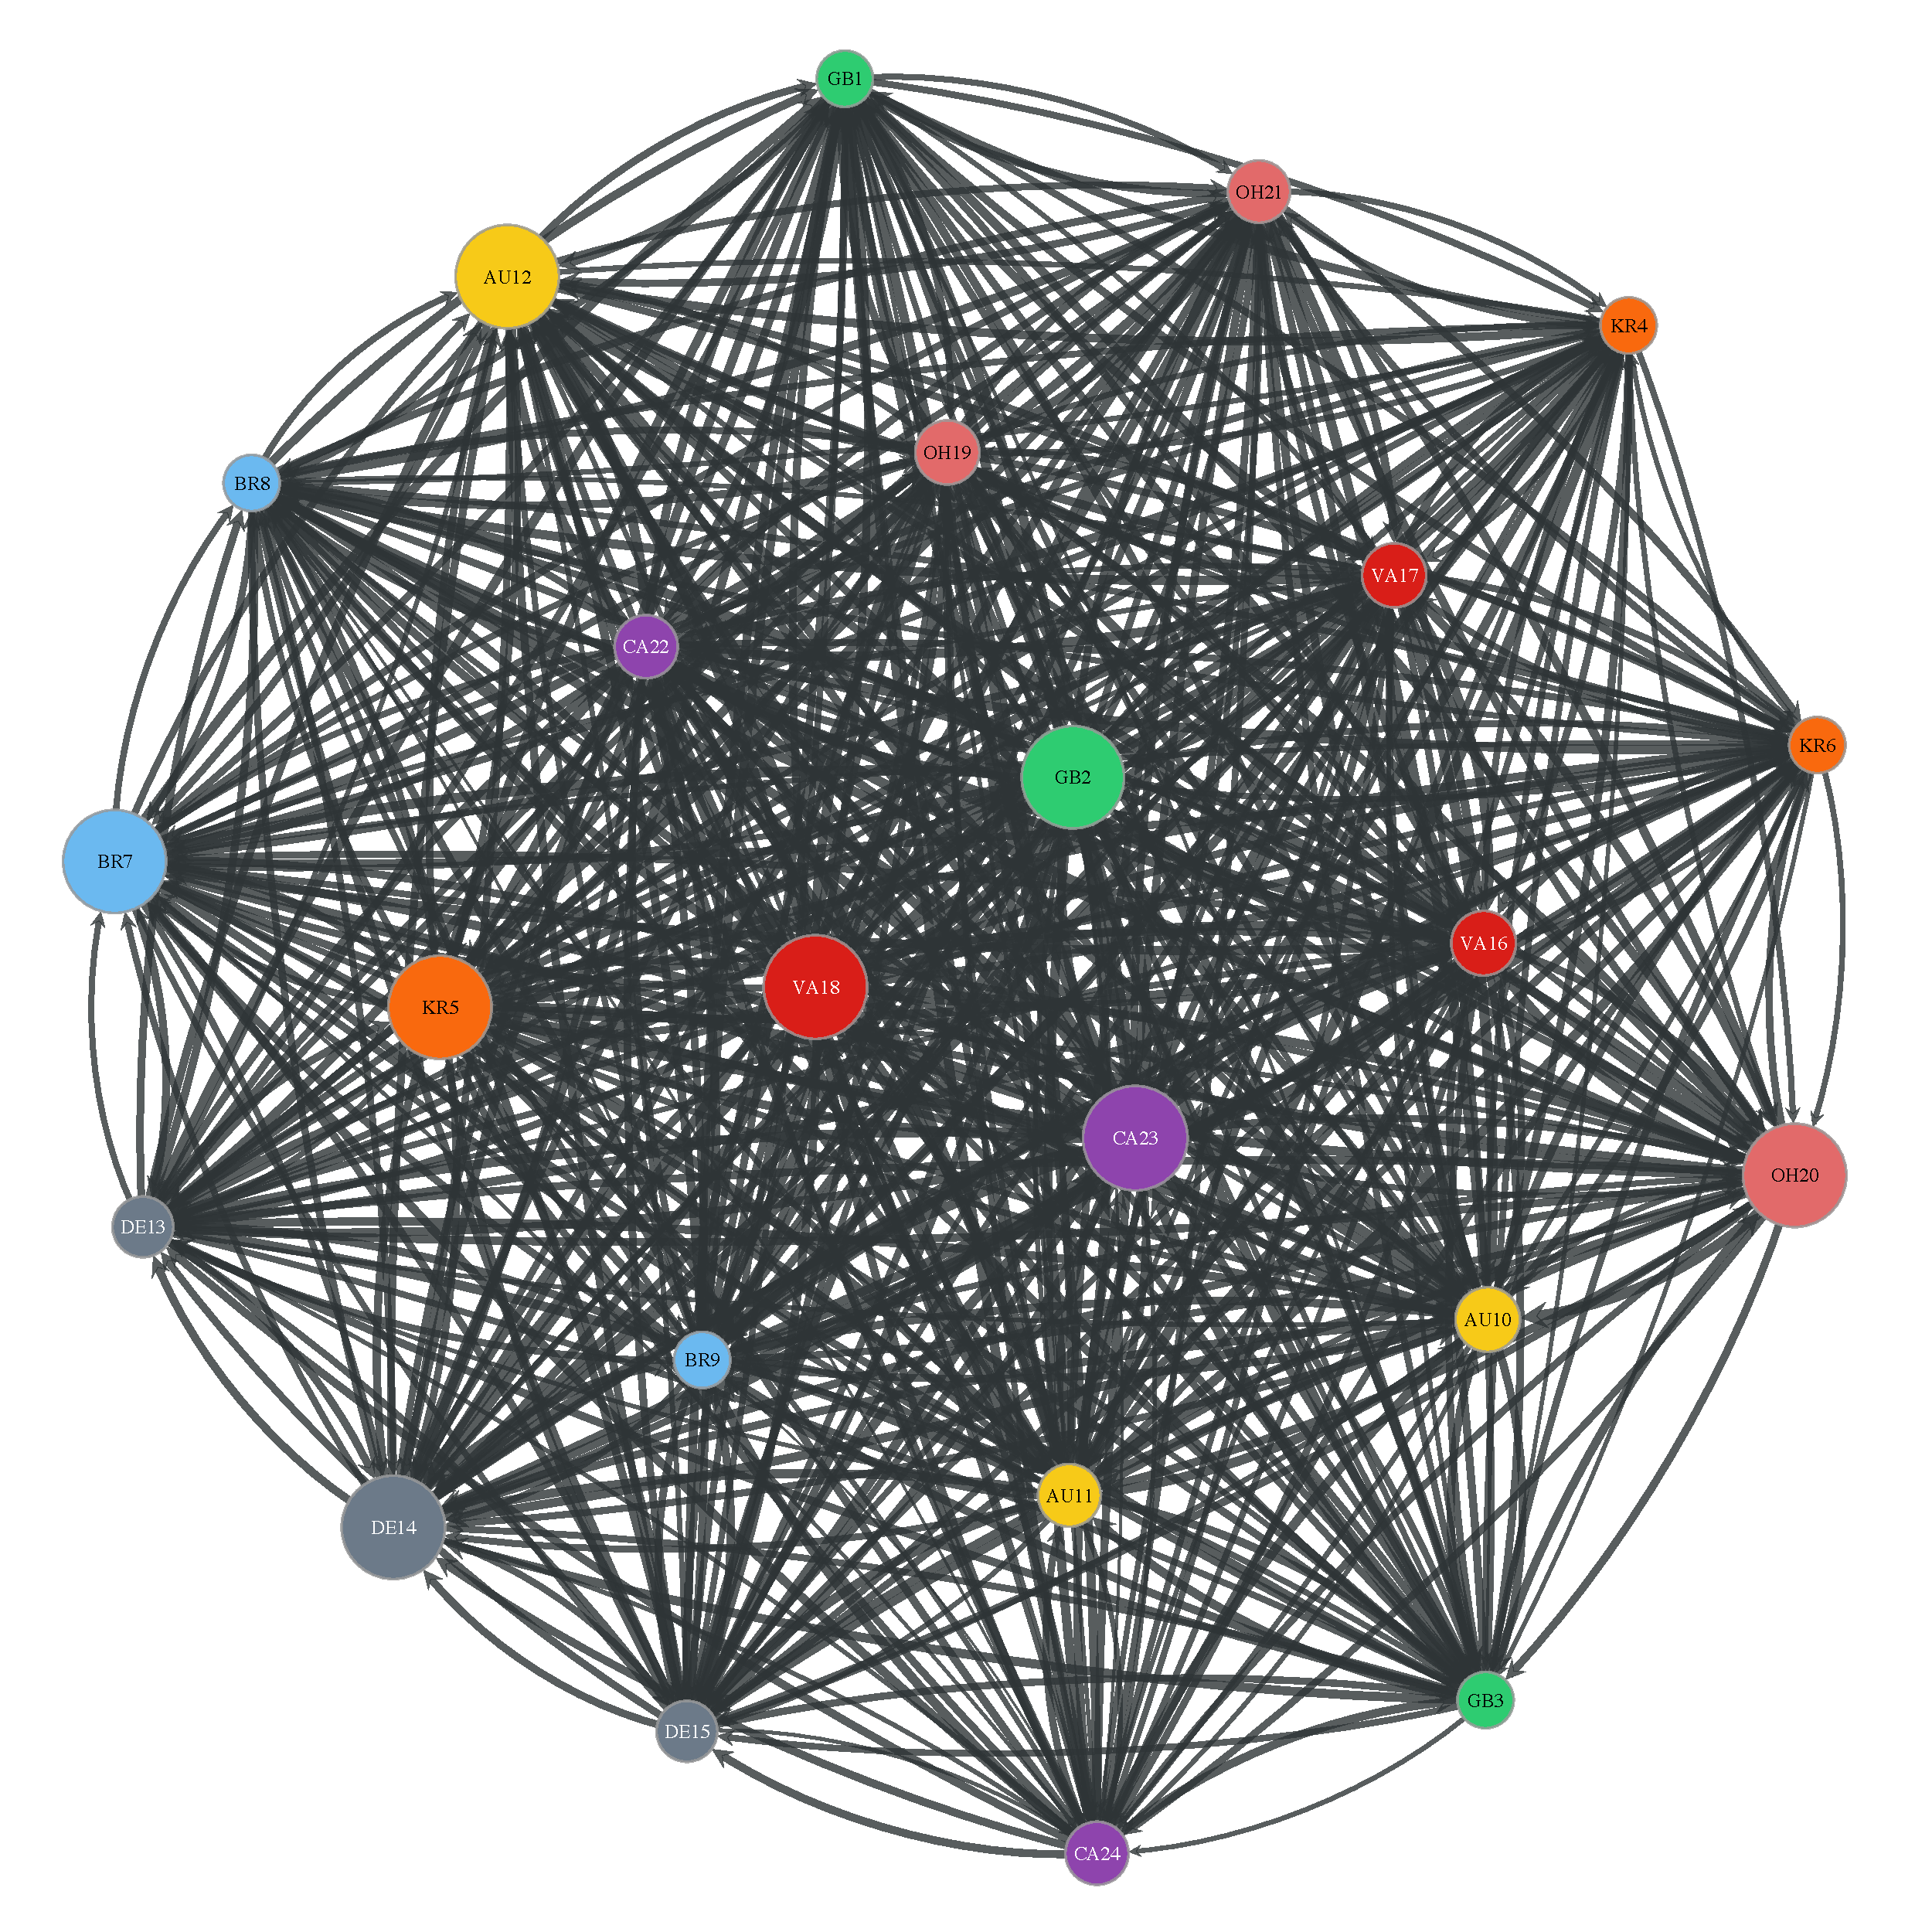
\includegraphics[width=\linewidth]{figures/b-uniform-selection-e1}
      \caption{Uniform Selection}\label{fig:uniform_selection}
    \endminipage\hfill
    \minipage{0.33\textwidth}%
      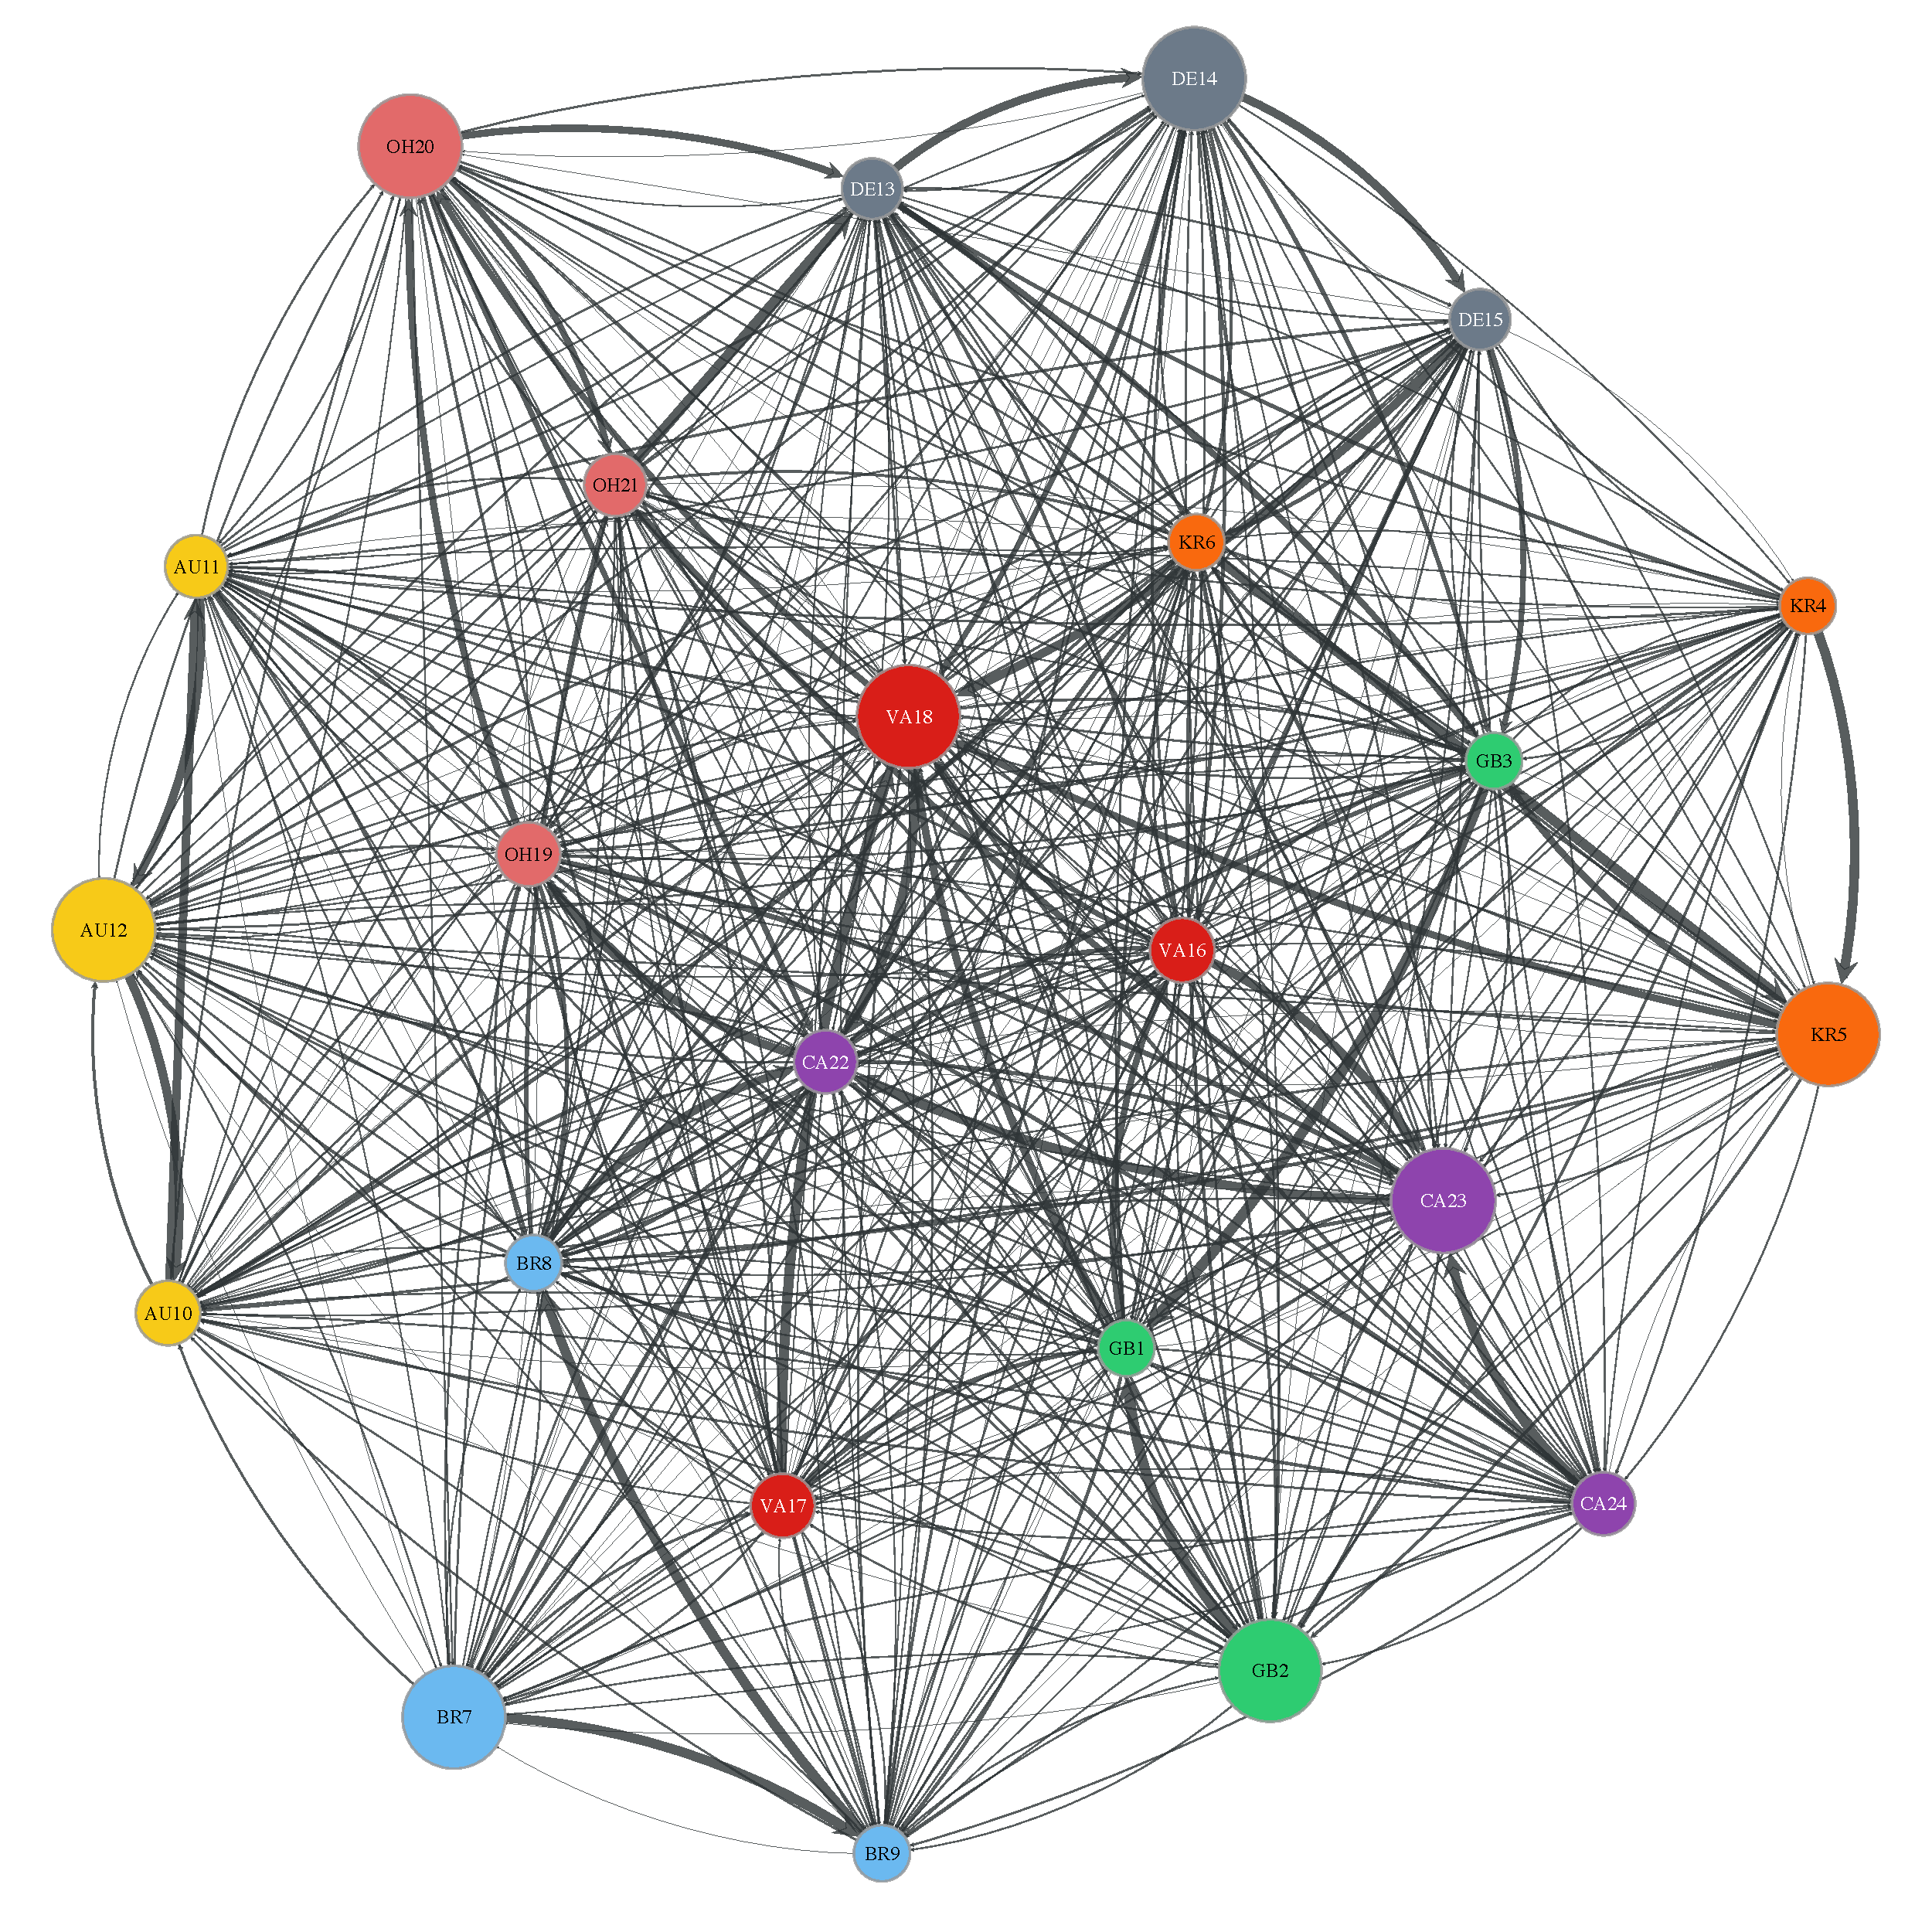
\includegraphics[width=\linewidth]{figures/b-annealing-epsilon-greedy-e5}
      \caption{Annealing Epsilon Greedy}\label{fig:annealing_epsilon}
    \endminipage\hfill
    \minipage{0.33\textwidth}%
      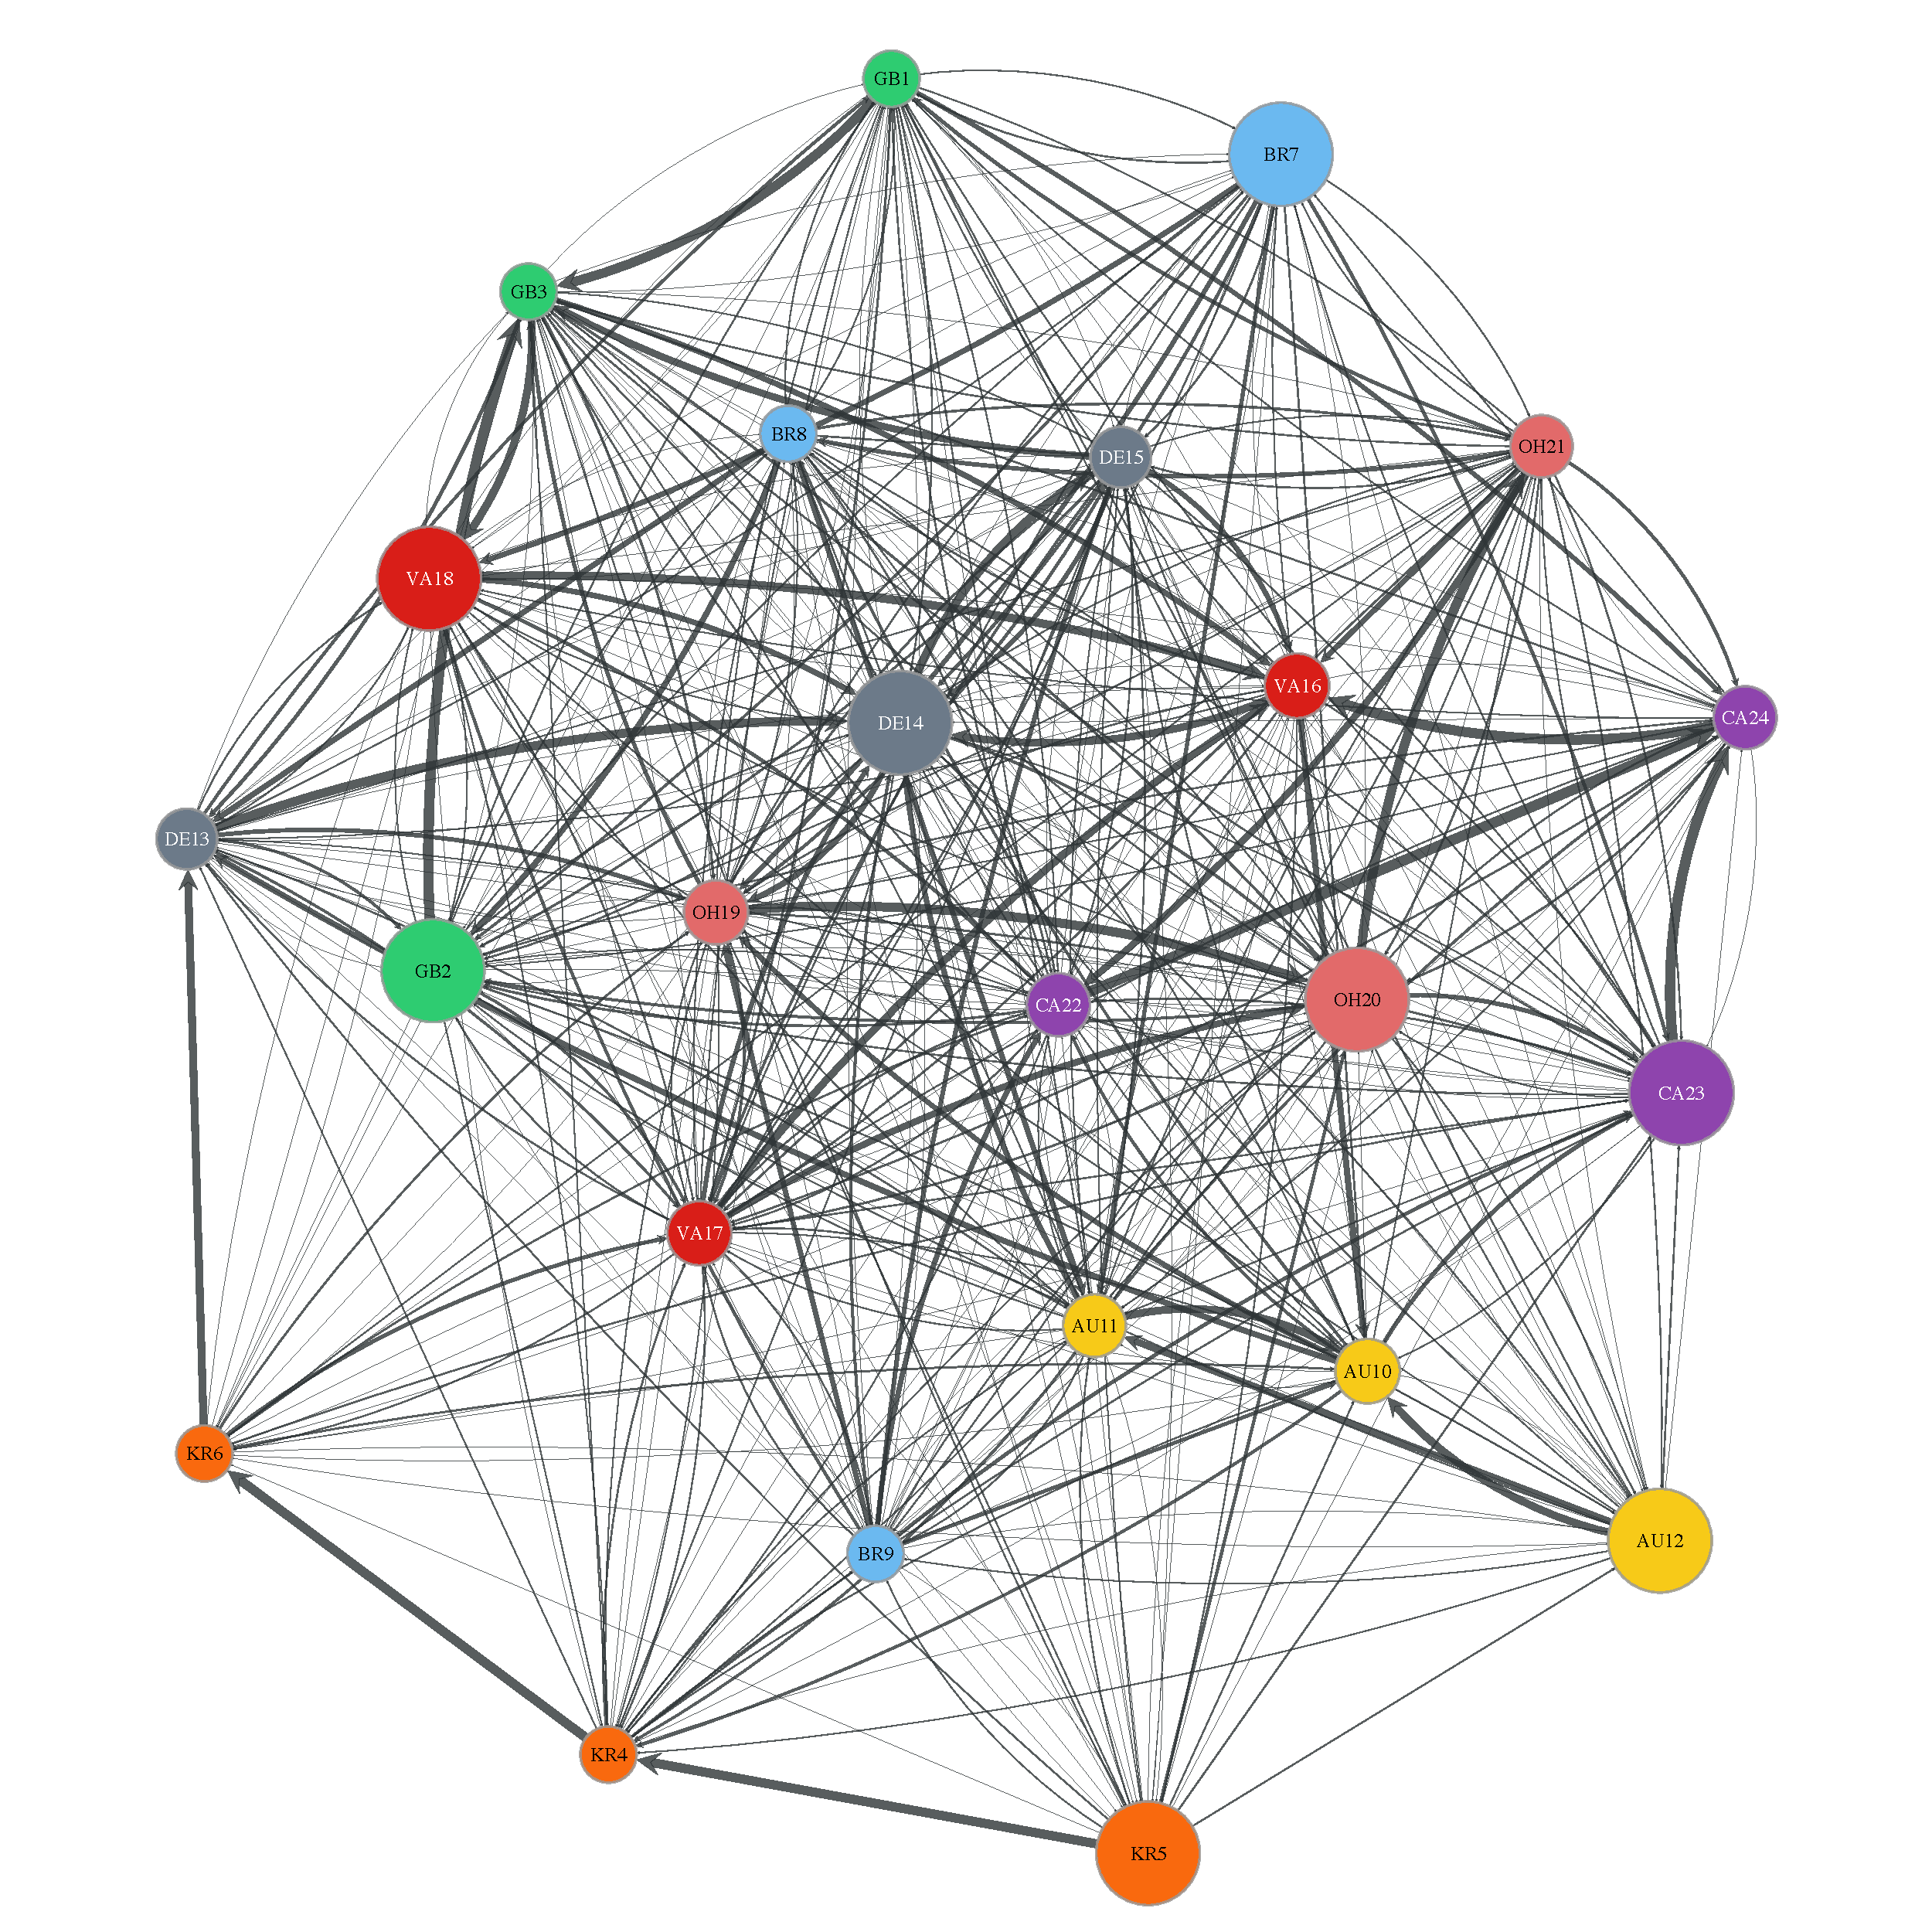
\includegraphics[width=\linewidth]{figures/b-epsilon-greedy-0-1-e2}
      \caption{Epsilon Greedy $\epsilon=0.1$}\label{fig:epsilon_greedy_e1}
    \endminipage
\end{figure*}

To show the emergent behavior of bandits, we have visualized the resulting
topologies as network diagrams in Figure~\ref{fig:uniform_selection} (uniform
selection), Figure~\ref{fig:annealing_epsilon} (annealing epsilon) and
Figure~\ref{fig:epsilon_greedy_e1} (epsilon greedy $\epsilon=0.1$).
Each network diagram shows each replica as a vertex, colored by region e.g.
purple is California, teal is Sao Paulo, Brazil, etc.
Each vertex is also labeled with the 2-character UN country or US state
abbreviation as well as the replica's precedence id.
The size of the vertex represents the number of \texttt{Put} requests that
replica received over the course of the experiment; larger vertices
represent replicas that were colocated with workload generators.
Each edge between vertices represents the total number of successful
synchronizations, the darker and thicker the edge is, the more
synchronizations occurred between the two replicas.
Edges are directed, the source of the edge is the replica that initiated
anti-entropy with the target of the edge.

Comparing the resulting networks, it is easy to see that more defined
topologies result from the bandit-based approaches.
The uniform selection network is simply a hairball of connections with
a limited number of synchronizations.
Clear optimal connections have emerged with the bandit strategies, dark
lines represent extremely successful synchronization connections between
replicas, while light lines represent synchronization pairs that are
selected less frequently.
We posit that fewer edges in the graph represents a more stable network;
the fewer synchronization pairs that are selected, the less noise that
occurs from selecting a peer that is in a similar state.

\section*{Discussion}

To achieve stronger eventual consistency, the visibility latency
of a system replicated with anti-entropy must be reduced.
We believe that this can be achieved with two primary goals: increasing
the number of successful synchronizations and maximizing the number
of local and regional synchronizations such that the average latency of
anti-entropy sessions is as low as possible.
These goals must also be tempered against other requirements, such as
fault and partition tolerance, a deterministic anti-entropy solution that
ensures the system will become consistent eventually, and load balancing
the synchronization workload evenly across all replicas.

Bandit based approaches to peer selection clearly reduce noise inherent
in uniform random selection as shown in Figure~\ref{fig:system_rewards}.
The bandit strategies achieve better rewards over time because peers
are selected that are more likely to have an update to synchronize.
Moreover, based on the network diagrams shown in
Figures~\ref{fig:uniform_selection}-\ref{fig:epsilon_greedy_e1}, this is
not the result of one or two replicas becoming primary syncs: most
replicas have only one or two dark in-edges meaning that most replicas
are only the most valuable peers for one or two other replicas.

Unfortunately, the rewards using a bandit approach, while clearly better
than the uniform case, are not significantly better -- this is an interesting
demonstration of the possibility of adaptive systems to improve consistency
but further investigation is required.
The primary place we see for adjustment is future work to explore the reward
function in detail.
For example, the inclusion of penalties (negative rewards) might make
the system faster to adjust to a high quality topology.
Comparing reward functions against variable workloads may also reveal a
continuum that can be tuned to the specific needs of the system.

As for localization, there does appear to be a natural inclination for
replicas that are geographically proximate to be a more likely selection.
In Figure~\ref{fig:epsilon_greedy_e1}, replicas in Canada (light blue),
Virginia (dark blue), Sydney (grey), California (purple), and Frankfurt
(light green) all prioritize local connections.
Regionally, this same figure shows strong links such as those between Ohio
and California (\texttt{CA42} $\rightarrow$ \texttt{OH38}) or Japan and
Singapore (\texttt{JP17} $\rightarrow$ \texttt{SG25}).
Replicas such as \texttt{BR19} and \texttt{IN3} appear to be hubs that
specialize in cross-region collaboration.
Unfortunately there does also seem to be an isolating effect, for example
Sydney (grey) appears to have no significant out of region synchronization
partners.
Multi-stage bandits might be used to create a tiered reward system to
specifically adjust the selection of local, regional, and global peers.
Other strategies such as upper confidence bounds, softmax, or Bayesian
selection may also create more robust localization.

Finally, and perhaps most significantly, the experiments conducted in
this paper were on a static workload; future work must explore dynamic
workloads with changing access patterns to more closely simulate real
world scenarios.
While bandit algorithms are considered online algorithms that do respond
to changing conditions, the epsilon greedy strategy can be slow to change
since it prefers to exploit high-value arms.
Contextual bandits use side information in addition to rewards to make
selection decisions, and there is current research in exploring contextual
bandits in dynamic worlds that may be applicable~\cite{luo_efficient_2017}.
Other strategies such as periodic reseting of the values may incur a small
cost to explore the best anti-entropy topology, but could respond to changing
access patterns or conditions in a meaningful way.

\section*{Conclusion}

In this paper we have presented a demonstration of adaptive consistency in
the geo-replicated eventually consistent systems by employing a novel
approach to peer selection during anti-entropy -- replacing uniform random
selection with multi-armed bandits.
Multi-armed bandits consider the historical reward obtained from
synchronization with a peer, defined by the number of objects synchronized
and the latency of RPCs, when making a selection.
Bandits balance the exploitation of a known high-value synchronization
peer with the exploration of possibly better peers or the impact of
failures or partitions.
The end result is a replication network that is less perturbed by noise
due to randomness and capable of more efficiently propagating updates.

In an eventually consistent system, efficient propagation of updates is
directly tied to higher consistency.
By reducing visibility latency, the likelihood of a stale read decreases,
which is the primary source of inconsistency in a highly available system.
We have demonstrated that bandit approaches do in fact lower visibility
latency in a large network.

This work, however, is preliminary.
Future efforts will consider different reward functions, different selection
strategies, dynamic environments, and how the priorities of system designers
can be embedded into rewards.
Reward functions that capture more information about the expected workload of
the system such as object size, number of conflicts, or localizing objects
may allow specific tuning of the adaptive approach.
We will also specifically explore in detail the effect of dynamic workloads
on the system and how the reinforcement learning can adapt in real time to
changing conditions.
We plan to investigate periodic resets, anomaly detection, and auction
mechanisms to produce efficient topologies that are not brittle as access
patterns change.
We also plan to evaluate other reinforcement learning strategies such as
neural or Bayesian networks to determine if they handle dynamic environments
more effectively.

% We believe that the next phase of consistency research will focus on a new
% class of adaptive distributed data systems that monitor their environment and
% modulate behavior in response to user access patterns, failures, and
% partitions in order to optimize a consistent global state.

We believe that the results presented show a promising start to a renewed
investigation of highly available distributed storage systems in novel
network environments, particularly those that span the globe.
Specifically, this work is part of a larger exploration of adaptive,
globally distributed data systems that federate consistency levels to provide
stronger guarantees~\cite{bengfort_federating_2017}.
Federated consistency combines adaptive eventually consistent systems such as
the one presented in this paper with scaling geo-replicated consensus such as
Hierarchical Consensus~\cite{bengfort_brief_2017} in order to create robust
data systems that are automatically tuned to provide the best availability
and consistency.
Distributed systems that adapt to and learn from their environments and
access patterns, such as the emerging synchronization topologies we observed
in this paper, may form the foundation for the extremely large, extremely
efficient networks of the future.

All code for the key-value store and bandit-based entropy as well as
experimental results is open source and available on GitHub at
\url{https://github.com/bbengfort/honu}.


\bibliographystyle{ACM-Reference-Format}
\bibliography{papers}

\end{document}
